% Created 2022-12-10 Sat 19:19
% Intended LaTeX compiler: pdflatex
\documentclass[preprint,numrefs,noinfo,sort&compress]{elsarticle}
  \usepackage[utf8]{inputenc}
\usepackage{url}
\usepackage[version=4]{mhchem}
\usepackage{chemmacros}[2016/05/02]
\usepackage{graphicx}
\usepackage{float}
\usepackage{color}
\usepackage{adjustbox}
\usepackage{amsmath}
\usepackage{siunitx}
\usepackage{textcomp}
\usepackage{wasysym}
\usepackage{latexsym}
\usepackage{amssymb}
\usepackage{lineno}
\usepackage{chemformula}
\usepackage{xr}
\usepackage{pifont}
\usepackage{longtable}
\usepackage[section]{placeins}
\usepackage{threeparttable}
\newcommand{\red}[1]{\textcolor{red}{#1}}
\chemsetup{formula = mhchem ,modules = {reactions,thermodynamics}}
\usepackage{xcolor}
\chemsetup[reactions]{tag-open= ( , tag-close = )}
\usepackage[capitalize]{cleveref}
\usepackage{minted}
\DeclareSIUnit\Td{Td}
\setminted[python]{frame=lines,fontsize=\scriptsize,xleftmargin=\parindent,linenos,breaklines}
\date{}
\title{}
\begin{document}

\frontmatter
\title{Characterization and Analysis of Ring Topology of Zeolite Frameworks}
\author[nd]{Jerry T. Crum}
\author[uoa]{Justin R. Crum}
\author[nd]{Cameron Taylor}
\author[nd,ndc]{William F. Schneider}
\address[nd]{Department of Chemical and Biomoledcular Engineering, University of Notre Dame, 250 Nieuwland Science Hall, Notre Dame, IN 46556, USA}
\address[uoa]{Department of Applied Mathematics, University of Arizona, 617 N Santa Rita Ave, Tucson, AZ 85721, USA}
\address[ndc]{Department of Chemistry and Biochemistry, University of Notre Dame, 251 Nieuwland Science Hall, Notre Dame, IN 46556, USA}
\begin{abstract}
The topology of zeolite frameworks and of associated tetrahedral sites (T-sites) are commonly characterized by their associated rings, typically defined as some set of closed paths or cycles through a framework that cannot be decomposed into shorter cycles. These ring descriptors have been used to identify feasible zeolite topologies, to describe the similarity and differences between zeolites, to identify sites or voids of catalytic relevance, and as machine learning fingerprints. Numerous definitions and algorithms for finding zeolite rings have been proposed and applied throughout the literature. Here we report an analysis of rings and T-sites in a large number of zeolite frameworks using Zeolite Simulation Environment, a Python package that implements an efficient algorithm presented by Goetzke and Klein for finding rings in arbitrary frameworks. We compare the result of a number of common and new ring definitions applied to a large number of common zeolite frameworks. We discover previously unrecognized rings in a number of frameworks. We show that the vertex symbol, a common approach used to characterize T-sites, misses important parts of the stereochemistry around a T-site, and propose an alternative definition. This tool provides an effective platform for characterizing zeolite and T-site structures useful for building models and doing machine learning.
\end{abstract}
\maketitle

\mainmatter
\section{Introduction}
\label{sec:org497996e}
Zeolites are three dimensional crystalline structures containing tetrahedral Si or Al atoms connected by oxygen bridges. The International Zeolite Association (IZA) lists over 200 known zeolite frameworks that are described by dimensionality, pore shape and size, and Si/Al ratios \cite{baerlocher-database-nodate}. It is natural to characterize differences in zeolites by the size and shapes of the features present in the crystal. Rings are one common type of feature widely reported and used, both to characterize a zeolite crystal and as descriptors of the individual tetrahedral sites (T-sites) of a zeolite. Rings have been used to identify feasible zeolites topologies \cite{li-why-2014}, to describe the similarity and differences between zeolites \cite{curtis-statistical-2003,bermudez-calculation-2017}, to identify sites or voids of catalytic relevance \cite{li-first-principles-2018,kester-effects-2021}, and as machine learning finger prints of physicochemical properties \cite{helfrecht-new-2019}. Rings can be used to describe the channel sizes for understanding shape selectivity in catalysis, zeolite building blocks for solid state chemists, and the sizes of framework cages and windows to provide insights into adsorption properties. The dimension and number of rings in a framework can be used to characterize entire zeolite frameworks, T-sites that make up these frameworks, or even the oxygen atoms that connect the T-sites. The number and dimension  of rings that pass through a T-site can be used to describe and differentiate the local void environment around symmetry distinct T-sites and to  differentiate symmetry distinct oxygen atoms. 

\begin{figure}
\begin{figure}[H]
\centering
\includegraphics[width=0.5\textwidth]{figures/chapter-3/ring-examples2.pdf}
\caption{Cutout of the Chabazite framework showing a path (5-6-7-8-9) highlighted with purple bonds, a cycle (3-4-18-19-20-17) highlighted with blue bonds, an 8-MR filled in with pink, and a 4-MR filled in with green. Yellow atoms are Si (T-sites), and red atoms are oxygen. \label{fig:3.1}}
\end{figure}
\end{figure}

A number of definitions and enumerations of rings in zeolites have been presented   \cite{guttman-ring-1990,goetzke-properties-1991,franzblau-computation-1991,yuan-efficient-2002-1,wooten-structure-2002,le-roux-ring-2010,sastre-zeotsites-2001} and implemented in software tools, including ZeoTSites \cite{sastre-zeotsites-2001} and ToposPro \cite{blatov-applied-2014}. Zeolites are naturally  represented using graph theory, in which  atoms are nodes and bonds are edges.  Because the oxygen atoms are only connected to exactly two T-sites, their inclusion in a graph does not change the graph structure, and thus T-sites can be  defined as nodes and the intervening oxygen atoms as edges \cite{goetzke-properties-1991}.  The cutout of the chabazite (CHA) framework shown in \cref{fig:3.1}  and  \cref{tab:graphs} summarize basic definitions of graphs that will be used here.  The size of each of these features can either be defined by the total number of atoms contained in them, or by the number of T-sites contained in them. The latter method is the standard convention, which we will use. A path is a sequence of edges that connects a sequence of nodes in which every edge is distinct (shown with purple highlighted bonds in \cref{fig:3.1}). A cycle is a path that starts and ends at the same node, and does not repeat any other nodes (shown by blue bonds in \cref{fig:3.1}). A zeolite crystal contains an infinite number of cycles, but the symmetry of the crystal reduces this to a finite number of symmetry-distrinct rings whose exact identity is subject to definition. \cref{fig:3.1} shows an 8-membered ring (8-MR) and a 4-MR filled in pink and green, respectively.

\begin{table}
\begin{threeparttable}
\caption{List of graph based features, their descriptions, and how they apply to frameworks, T-sites, and oxygen atoms. \label{tab:graphs}}
{\tiny
\begin{tabular}{lp{1.5cm}p{2cm}p{2cm}p{2cm}}
\hline
Feature & Description & Application to Frameworks & Application to T-sites & Application to Oxygen Atoms\\
\hline
Node & T-site or oxygen atom & Contains some set of symmetry distinct nodes &  & \\
Path & A sequence of nodes that are connected to each other & Traverses through a framework & T-sites and oxygen atoms connected in series forms a path & T-sites and oxygen atoms connected in series forms a path\\
Cycle & A path that starts and ends at the same node, and does not repeat any other nodes & Contains some set of cycles & Formed by alternating connected T-sites and oxygen atoms & Formed by alternating connected T-sites and oxygen atoms\\
Rings & A cycle that does not contain a shortcut \cite{guttman-ring-1990,goetzke-properties-1991} & Can describe channels of a framework, or other distinct void environments & Can be described by counting the number of rings that pass through it & Can be described by the number of rings that pass through it\\
Modified Shortcut Rings & A cycle that does not contain a modified shortcut & A subset of the rings will be found in the framework & Used to describe a T-site & Used to describe an oxygen atom\\
Shortest Path Rings & A ring that is the shortest ring for at one least one set of O-T-O along the cycle & Another subset of the rings of a framework & Used to describe a T-site & Used to describe an oxygen atom\\
Vertex Symbol Rings & The rings making up the vertex symbol of a T-site & Yet another subset of the rings of the framework & Used to describe a T-site & Not applicable to oxygen atoms\\
\hline
\end{tabular}

\begin{tablenotes}
}
\end{tablenotes}
\end{threeparttable}
\end{table}

% These rings are relevant to ion exchange and shape selectivity in catalysis, to describing the zeolite building blocks relevant to zeolite assembly, and to capturing void spaces relevant to  adsorption properties. 

 In the most basic definition, a ring is any cycle that does not contain any shortcuts \cite{guttman-ring-1990,goetzke-properties-1991}.  A shortcut is defined as a path connecting two nodes of a cycle that decomposes the cycle into smaller rings \cite{guttman-ring-1990,goetzke-properties-1991}; i.e., a path is a shortcut if it is shorter than both paths between these nodes along the cycle. An example is the path connecting T17 and T18 in \cref{fig:3.1}, which is a shortcut of the blue cycle. This path contains two T-sites, splitting the 8-MR cycle into two 4-MRs. While general, this definition reports, as distinct, ring features of a zeolite framework that do not intuitively relate to local structure, accessibility, or usefully ``fingerprint'' frameworks. Thus, more restrictive defintions of zeolite rings have been proposed. For instance, a ``strong ring'' is defined as a ring that is not the sum of a set of smaller rings \cite{goetzke-properties-1991,blatov-three-periodic-2007}.

 Another method for pruning the list of rings found in a zeolite frameworks is based off of the concept of a vertex symbol. The vertex symbol is a common way to describe the structure around the T-sites of zeolite frameworks and was first used to do so in 1997 by O'Keeffe and Hyde \cite{okeeffe-vertex-1997}. The vertex symbol of a T-site is determined by the shortest rings associated with each of the six edges of the tetrahedron formed by the T-atom and its four bound oxygen atoms. The symbol is formed by grouping rings on opposite edges of the tetrahedron and listing from smallest to largest. \cref{fig:cha-vertex}(a) shows as example the tetrahedron formed at the single symmetry-distinct T-site in the CHA framework. The edges of the tetrahedron are labeled to aid in identification. \cref{fig:cha-vertex}(b-d) show the rings associated with each opposite pair of edges. The vertex symbol of T1 in CHA is thus 4\(\cdot\)4\(\cdot\)4\(\cdot\)8\(\cdot\)6\(\cdot\)8. For a T-site that contains a multiplicity of rings at one edge, that multiplicity would be represented as a subscript in the vertex symbol. An example would be the vertex symbol of 4\(\cdot\)6\(_{\text{2}} \cdot\)6\(\cdot\)6\(_{\text{3}} \cdot\)6\(_{\text{2}} \cdot\)6\(_{\text{3}}\) for T1 in AFI.  The rings of a framework are then the union of the rings of all the distinct T-sites, a definition that eliminates some rings that satisfy the no shortcut criterion. 

\begin{figure}
\begin{figure}[H]
\centering
\includegraphics[width=\textwidth]{figures/chapter-3/cha-vertex.pdf}
\caption{Cutout of the CHA framework, showing the rings that make up the vertex symbol of the single symmetry distinct T-site. a) Example of the tetrahedron formed by the T-site and four connected oxygen atoms, with labeled edges of the tetrahedron. b) Rings associated with opposite edges E1 and E3. c) Rings associated with opposite edges E5 and E6. d) Ring associated with opposited edges E2 and E4. Rings are colored as: 4-MR (green), 6-MR (blue), and 8-MR (pink). \label{fig:cha-vertex}}
\end{figure}
\end{figure}

Sastre and Corma \cite{sastre-topological-2009} proposed an alternative convetion, in which distinct rings are only those that form the shortest cycle connecting any \ce{O-T-O} in a framework. This convention provides an univocal count of the rings that pass through a T-site without the ambiguity of limiting the search to a certain ring size. Using AFI as an example,  (\cref{fig:3.3}(a)) shows that both a 12-MR (purple) and a 6-MR (blue) pass through the labeled T1 atom. The 12-MR would not be included in the Sastre and Corma enumeration because for every \ce{O-T-O} along the 12-MR, the shortest path connecting them is not the 12-MR. The difference between this criterion and the vertex symbol rings is subtle, but with this shortest path convention any ring belonging to the vertex symbol of any T-site in a framework will be included in the ring count for each of the T-sites that ring passes through. \cref{fig:3.4} shows a cutout of the TON framework including a 6- (blue) and 10-MR (orange). For T1, only the 6-MR would be counted within the vertex symbol convention because it is the shortest path connecting O2 and O3. The 10-MR is the shortest path connecting O2, and since this 10-MR is the shortest path for at least one set of \ce{O-T-O} along the cycle, and passes through T1, it does get counted in the shortest path rings for T1.

\begin{figure}
\begin{figure}[H]
\centering
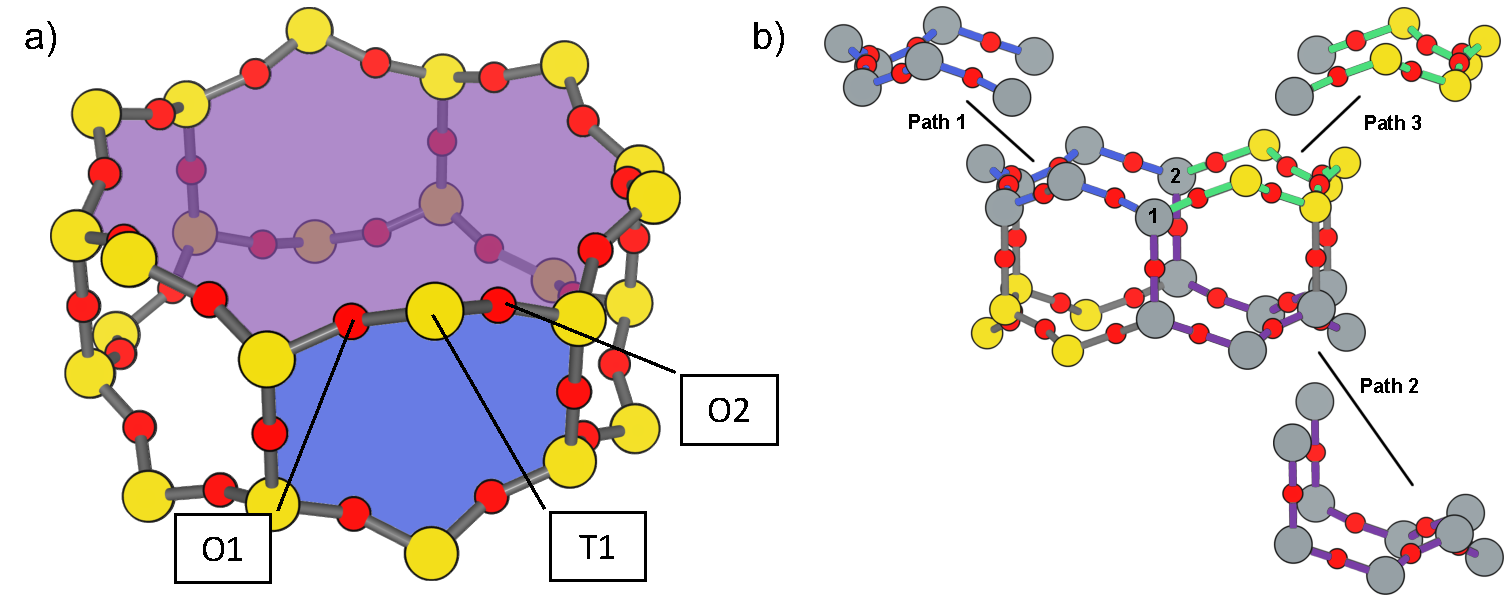
\includegraphics[width=\textwidth]{figures/chapter-3/afi-14-and-modified.pdf}
\caption{Cutouts of the 12-MR channel in AFI: a) Highlighting a 12-MR in purple, and a 6-MR in blue. The 6-MR is included in the vertex symbol of labeled T1 because it is the shortest path connecting O1 and O2. The 12-MR would not be included in the vertex symbol or shortest path ring list because for each O-T-O along the 12-MR there is a shorter path connecting them. b) A 14-MR is shown as T-sites replaced with aluminum atoms in gray. The two paths connecting Al1 and Al2 that make this 14-MR are highlighted with blue and purple bonds. Path 3 highlighted with green bonds is a modified shortcut connecting Al1 and Al2. \label{fig:3.3}}
\end{figure}
\end{figure}

% The vertex symbol is a property of a T-site that is determined by the rings that pass through that site. Because the vertex symbol convention  lists rings in an order determined by size and locations on opposite edges of the tetrahedron, it is possible for two T-sites of differing connectivity (effectively, local constitutional isomers) to be described by the same  vertex symbol
% The ring sizes, and  their multiplicity, for opposite edges (edges of the tetrahedron that do not connect to the same oxygen atom) are grouped together. These grouped pairs are listed from smallest to largest forming the vertex symbol.
%  the number and type of rings Because various conventions exist that can reduce the set of rings in a zeolite to more strictly defined properties, the ring counts returned by the various conventions will differ. Differences in ring counts leads to differences in how one might describe the topological environment of a zeolite. Therefore, when using rings to describe the properties of a framework, T-site, or oxygen atom, it is of value to characterize the differences between the conventions and to have a use one that determines the features of interest.  

\begin{figure}
\begin{figure}[H]
\centering
\includegraphics[width=0.5\textwidth]{figures/chapter-3/ton-6-10.pdf}
\caption{Cutout of the TON framework showing a 6- (blue) and 10-MR (orange). The 10-MR is the shortest path connecting O14-T3-O2, and passes through T1, so it is counted in the shortest path rings for T1. \label{fig:3.4}}
\end{figure}
\end{figure}


Thus, the dimensions and numbers of rings present in a framework will differ depending on precise convention, with potential consequences for the ability to relate properties to rings. Here we present an analysis of rings captured by Goetzke and Klein's efficient ring finding algorithm \cite{goetzke-properties-1991} and compare those rings to the rings found by other previously published ring set reduction conventions. We have implemented all of these ring finding conventions in a Python package called the Zeolite Simulation Environment (ZSE) \cite{crum-jtcrumzse-2022}. We use ZSE to analyze the sets of rings captured by each convention across the entire set of zeolite frameworks contained in the IZA Database \cite{baerlocher-database-nodate}. We  highlight rings that are found by these conventions but not typically discussed in the literature for a number of frameworks. A comparison of the rings reported by various conventions to those listed in the IZA highlights differences related to fused rings illustrated in \cref{fig:3.3}}b. We propose a modification of the shortcut definition that results in a set of rings closer to those listed in the IZA database than do existing conventions.  Lastly, we consider the vertex symbol \cite{okeeffe-vertex-1997} characterization of T-sites and show that T-sites described by the same vertex symbol are not necessarily superimposable but rather can have distinct local stereochemistries.  We identify and enumerate these cases of constitutional isomerization within T-sites of identical vertex symbol and propose an alternative convention that uniquely takes into account their orientation and connectivity around the T-site.

\section{Methods}
\label{sec:org568c810}

\subsection{Rings That Do Not Contain Shortcuts \label{section:goetzke}}
\label{sec:orgeb1d79d}

We implemented the efficient algorithm presented by Goetzke and Klein \cite{goetzke-properties-1991} in ZSE \cite{crum-jtcrumzse-2022} to find all the rings associated with a T-site that do not contain a shortcut. In ZSE we use the framework put in place by the Atomic Simulation Environment (ASE) \cite{hjorth-larsen-atomic-2017} to handle routine analysis zeolite crystal structures. All graph theory functions are performed using the NetworkX Python package \cite{hagberg-exploring-2008}. 

First, we convert the ASE atoms object into a connectivity matrix which represents every atom across the columns and rows. If two atoms are bound together, their respective entry in the connectivity matrix contains a 1, else a 0. This connectivity matrix is then converted to a NetworkX graph object, and then a distance dictionary using NetworkX built in functions. Then we implement Step 3 from Geotzke and Klein's algorithm \cite{goetzke-properties-1991} summarized here: to find the rings that pass through a T-site, we iteratively search for every size ring between 3-MR and a maximum ring value that is user-specified. For this work we set a cutoff of 18-MRs. A schematic showing the evolution of the ring search is shown in \cref{fig:goetzke}. For ring size \(\lambda\) we start at the T-site of interest (labeled 1), and search the distance matrix for any T-sites that are \(\lambda\)/2 (even \(\lambda\)) or (\(\lambda\)-1)/2 (for odd \(\lambda\)) distance from the starting T-site (labeled 2). Next we attempt to create two distinct paths from 1 \(\rightarrow\) 2 and from 2 \(\rightarrow\) 1 alternating adding a node to each path as indicated by \cref{fig:goetzke}. Each node added to each of the paths must be \(\lambda\)/2 (even \(\lambda\)) or (\(\lambda\)-1)/2 (odd \(\lambda\)) from the head of the other path. Also each node added to each path needs to be the correct distance from 1 and 2 for the given step respectively. If either of the previous two conditions are not met, a ring cannot be formed of length \(\lambda\) along the given paths, we backtrack and repeat until all possible options have been explored for \(\lambda\). Then we increase \(\lambda\) and continue until the cutoff ring size is completed.

\begin{figure}
\begin{figure}[H]
\centering
\includegraphics[width=0.5\textwidth]{figures/chapter-3/goetzke.pdf}
\caption{Diagram showing how the ring finding algorithm evolves. Adapted from Goetzke and Klein \cite{goetzke-properties-1991}. \label{fig:goetzke}}
\end{figure}
\end{figure}

\subsection{Vertex Symbol Rings \label{section:vertex}}
\label{sec:org415adcd}

Starting from the set of all rings found in \cref{section:goetzke}, we prune the ring list to the set of vertex symbol rings. We find the shortest ring in the set that connects each pair of oxygens bound to our initial T-site. It is possible for there to be multiple rings of the same size connecting each oxygen, in which case all the rings of that size are kept. 

\subsection{Shortest Path Rings}
\label{sec:org6be3a64}

We prune the set of all rings from \cref{section:goetzke} to a subset of rings the meets the shortest path definition published by Sastre and Corma \cite{sastre-topological-2009}. For each ring, we iterate over every group of \ce{O-T-O} atoms in the ring, and check whether this ring is the shortest path connecting the two oxygen atoms. If so, the loop is broke, because the ring need only be the shortest path for one group of \ce{O-T-O} atoms to fit the definition. This is the most time consuming process out of all the ring finding conventions we have implemented.

\subsection{Modified Shortcut Rings \label{section:modified}}
\label{sec:org9232478}
The shortest path convention generally finds fewer (and smaller) rings than does an all non-shortcut bearing ring convention. As we show below, these two conventions bracket the set of rings captured in the IZA Structure Database, the all-rings convention generally including even larger rings and the shortest path convention missing large rings.
In seeking a convention of intermediate stringency, we identified a convention that would require the shortcut to be shorter than one, rather than both, of the paths connecting two nodes along the ring. This modified shortcut definition is illustrated in \cref{fig:3.3}(b).  By the standard shortcut convention, AFI would be considered to contain a 14-MR formed from the union of Path 1 (blue) and Path 2 (purple) through T1 and T2. However, because T1 and T2 are also connected by Path 3, which, while the same length as Path 1, is shorter than Path 2, the 14-MR does not satisfy the modified shortcut criterion. As we show below, the modified shortcut rule identifies rings of a given zeolite that are closer to those identified in the IZA Structure Database as rings of interest than do either all-ring or shortest-path-ring rules. 

Algorithmically, to remove rings containing modified shortcuts from the full set of rings, we iterate over every T-site pair of the ring and check for the shortest path connecting them. If that shortest path is shorter than either of the two paths along the ring connecting the two T-sites, we check whether the combination of this shorter path and the shorter of the two ring paths forms a new smaller ring. If so the iteration is broken, and the ring is removed from the counted set. 

\subsection{Ordered Vertex Symbols \label{section:ov}}
\label{sec:org7db42da}

To add information about the spatial orientation of the rings around a T-site to the vertex symbol, we have developed a method to order the edges in the vertex symbol. We systematically list the rings by following the edges of the tetrahedron such that each ring listed is connected to one of the oxygens of the next ring listed. After removing all the rings that are not a part of the vertex symbol (\cref{section:vertex}) we use the following process to order them. 

\begin{enumerate}
\item List all the possible arrangements of the oxygens bound to the T-site (4! = 24 possible arrangements).
\item Use a predetermined order of edges: [[0,2],[0,1],[1,2],[2,3],[3,0],[1,3]].
\begin{enumerate}
\item Where each of those values represents the index of the oxygen to use.
\end{enumerate}
\item Find the ring size (and multiplicity) connecting each pair of oxygens in this predetermined order.
\item Make a list of weights, where for each pair of oxygens the weight is the ring size \texttimes{} multiplicity.
\item Reverse sort the list of all possible oxygen arrangements by the correlating list of weights.
\item Use the first oxygen arrangement coupled with the predetermined edge order to list the rings and multiplicity for each edge.
\end{enumerate}

\subsection{Determining All Ring Sizes Contained in a Zeolite Framework}
\label{sec:org6a29aa7}



Finally, to determine all the ring sizes exhibited with in a zeolite framework, we take advantage of T-site symmetry. The rings of a framework are made of T-sites, and if two T-sites are symmetrically identical they will have the same set of rings passing through them. Therefore, we only need to find the rings associated with each symmetry distinct T-site to know all the possible ring sizes within a framework. For example, AFI only contains one symmetry distinct T-site (T1). Using the basic definition of a shortcut, T1 is a part of 4-, 6-, 12-, and 14-MRs when using a cutoff of 18-MR. Every other T-site in the AFI framework is also a T1, thus the only possible ring sizes in AFI are 4-, 6-, 12-, and 14-MRs.

\section{Results}
\label{sec:org47268f3}
\subsection{Characterizing Rings in a Zeolite Graph}
\label{sec:orgdbc479c}
The IZA Database \cite{baerlocher-database-nodate} is a common reference used to identify all the rings in a zeolite framework, however it only lists the rings that define a channel (ex: 12-MR in AFI), or rings associated with the symbol of a T-site. These rings listed by the IZA are referred to as tabulated rings in the literature \cite{curtis-statistical-2003}. In some frameworks, other rings (cycles not containing shortcuts) exist that are not included in the list of tabulated rings. These 'untabulated' rings may still provide important topological information about a zeolite framework, or the local void environment around a T-site. \cref{fig:fw-counts} shows counts of frameworks containing each size ring from 3- to 18-MR using the Goetzke algorithm and the listed rings on the IZA database \cite{baerlocher-database-nodate}. There are slight differences in the counts up to 6-MRs, but the main divergence takes place as we get to ring sizes \textgreater6-MR. We have limited our search to 18-MR because the differences in ring finding conventions are captured with the smaller rings, requiring less computation time, and there is a lower probability of finding larger rings in zeolites \cite{li-why-2014}.

\begin{figure}
\begin{figure}[H]
\centering
\includegraphics[width=\textwidth]{figures/chapter-3/rings-vs-iza-rings.pdf}
\caption{Counts of IZA frameworks containing each size ring between 3- and 18-MR using the Goetzke algorithm and the tabulated rings listed by the IZA \cite{baerlocher-database-nodate}. \label{fig:fw-counts}}
\end{figure}
\end{figure}

Taking a closer look at some of these untabulated rings highlights rings not typically listed for some frameworks, but are still relevant to describing their topology. Using CHA as an example, \cref{fig:cha-rings} displays a 12-MR (in purple) that circumferences the CHA cage. This ring is not associated with the vertex symbol of the single symmetry distinct T-site in CHA and does not define a channel. Thus, this ring is not included in the list of tabulated rings. We would argue that this is still a ring that provides an important topological descriptor of CHA because none of the tabulated rings provide information about the size of the CHA cage. 

\begin{figure}
\begin{figure}[H]
\centering
\includegraphics[width=\textwidth]{figures/chapter-3/cha-all-rings.pdf}
\caption{Chabazite cage and double 6-MR (D6R) with highlighted rings: 4-MR in green, 8-MR in pink, and 12-MR in purple. The 8-MR in the D6R and the 12-MR are rings not typically discussed in literature. Si atoms have been replaced with Al atoms to help identify those rings in the overal cage strcuture. \label{fig:cha-rings}}
\end{figure}
\end{figure}

Using AFI as another example, we find another type of ring that arises from traversing a pair of stacked rings and is not included in the list of tabulated rings. AFI, like CHA, contains one symmetry distinct T-site. According to the IZA, the AFI framework contains 4-, 6-, and 12-MRs \cite{baerlocher-database-nodate}. When we search for rings using the Goetzke algorithm \cite{goetzke-properties-1991}, we also find that it contains 14-MRs created by using seven T-sites from two 12-MRs that are separated by a distance of one oxygen (\cref{fig:afi-14}). Rings of this nature are prevalent in many frameworks; another example can be seen in the bottom right of \cref{fig:cha-rings}, where an 8-MR is highlighted traversing the two 6-MRs of the D6R. These types of rings may not be of interest depending on which topological feature one intends to describe. This has led us to create a modified definition of a shortcut as explained in \cref{section:modified}, which excludes these types of rings. The benefit of this new shortcut definition is that larger rings that are missed by the vertex symbol or shortest path rings (i.e., 12-MR in AFI) are still captured, while excluding rings that arise from convolution of stacked rings found with the typical shortcut definition.

\begin{figure}
\begin{figure}[H]
\centering
\includegraphics[width=\textwidth]{figures/chapter-3/afi-14.pdf}
\caption{Cutout of the 12-MR channel in AFI with a 14-MR (yellow) traversing seven T-sites of each 12-MR. The T-sites comprising the 14-MR have been replaced with Al for visibility. \label{fig:afi-14}}
\end{figure}
\end{figure}

\subsection{Characterizing Frameworks by Rings}
\label{sec:org3c3c2d3}
With the addition of our modified shortcut definition, we can compare the results of four ring finding conventions to the tabulated rings listed in the IZA Database. \cref{fig:ring-counts} shows how many frameworks contain each size ring found using the various ring counting conventions from 3- to 18-MRs. This plot highlights the differences in the conventions and shows that a topological description of a framework based on rings will depend on the way that you define a ring. In general, a hierarchy of ring sizes found by each convention is: all rings not containing a shortcut \textgreater this work \textgreater shortest path rings \textgreater vertex symbol rings. The IZA listed rings include the vertex symbol rings, and a selection of general rings \cite{baerlocher-database-nodate}.  

\begin{figure}
\begin{figure}[H]
\centering
\includegraphics[width=\textwidth]{figures/chapter-3/ring-counts-2.pdf}
\caption{Number of IZA zeolite frameworks containing each size ring, using the various ring counting conventions, as well as the rings listed by the IZA Database \cite{baerlocher-database-nodate}. \label{fig:ring-counts}}
\end{figure}
\end{figure}

One drawback to using a ring convention based on connectivity and shortcuts is the exclusion of non-ring cycles that exhibit geometric properties similar to those designated as rings. This is a trade-off between well-defined connectivity rules, and the inclusion of particular void environments that may still have important applications. These shortcut containing cycles can display chemical and/or geometric properties consistent with rings and are of interest to catalysis researchers even though they are not classically considered rings. One example is the 6-membered cycle referred to as the \(\alpha\)-6-MR in literature (\cref{fig:mfi-6}) and is present in a number of frameworks including but not limited to MOR, FER, MFI, and BEA \cite{dedecek-siting-2012,bernauer-proton-2016}. This \(\alpha\)-6-MR is a potential location for Co\(^{\text{2+}}\) uptake when two Al atoms are 3rd nearest neighbor (NN) in the cycle  \cite{bernauer-proton-2016,nimlos-experimental-2020}, similar to Co\(^{\text{2+}}\) uptake at 3NN Al atoms in 6-MRs in other frameworks such as CHA \cite{di-iorio-cooperative-2020}. \cref{fig:mfi-6} shows that this particular structure would be considered two 5-MRs using connectivity rules based on a shortcut. 

\begin{figure}
\begin{figure}[H]
\centering
\includegraphics[width=\textwidth]{figures/chapter-3/MFI-6MC.pdf}
\caption{Cutout of MFI framework showing the structure referred to as an \(\alpha\)-6-MR in blue, and the two 5-MRs that compose it in green. The 6-membered cycle would not be found by any of the connectivity ring rules outlined in this work. \label{fig:mfi-6}}
\end{figure}
\end{figure}

\subsection{Characterizing T-sites by Rings}
\label{sec:org6b7283b}

Considering that zeolite frameworks are comprised of one or more symmetry distinct T-sites, it may be of interest to describe those T-sites by the rings that pass through them. Most often the vertex symbol is used to make such a classification \cite{okeeffe-vertex-1997}. Sastre and Corma also provided characterization of T-sites using the shortest path rings that pass through them \cite{sastre-topological-2009}. In their work, they presented the ring index, which lists all the rings passing through a T-site from smallest to largest, and a subscript for each size representing it's multiplicity.  The rings associated with a T-site can provide information about the local void environments around the T-site, and could potentially be correlated to other physicochemical properties of the T-site once sufficient data on those physicochemical properties exists. 

Take for example the AFI framework, containing one symmetry distinct T-site. AFI contains 4-, 6-, 12-, and 14-MRs. To describe that T-site we can count how many of each of those rings pass through the T-site. We can also prune this list using our modified definition of a shortcut, the shortest path rings definition \cite{sastre-topological-2009}, or the rings contained within the vertex symbol of this T-site \cite{okeeffe-vertex-1997}. Using the ring index outlined above, each of these conventions will provide a different description of the zeolite (highlighted in \cref{fig:afi-funnel}):
\begin{itemize}
\item Rings: 4\(\cdot\)6\(_{\text{13}} \cdot\)12\(\cdot\)14\(_{\text{7}}\)
\item This work: 4\(\cdot\)6\(_{\text{13}} \cdot\)12
\item Shortest Path Rings: 4\(\cdot\)6\(_{\text{13}}\)
\item Vertex Symbol Rings: 4\(\cdot\)6\(_{\text{11}}\)
\end{itemize}

\begin{figure}
\begin{figure}[H]
\centering
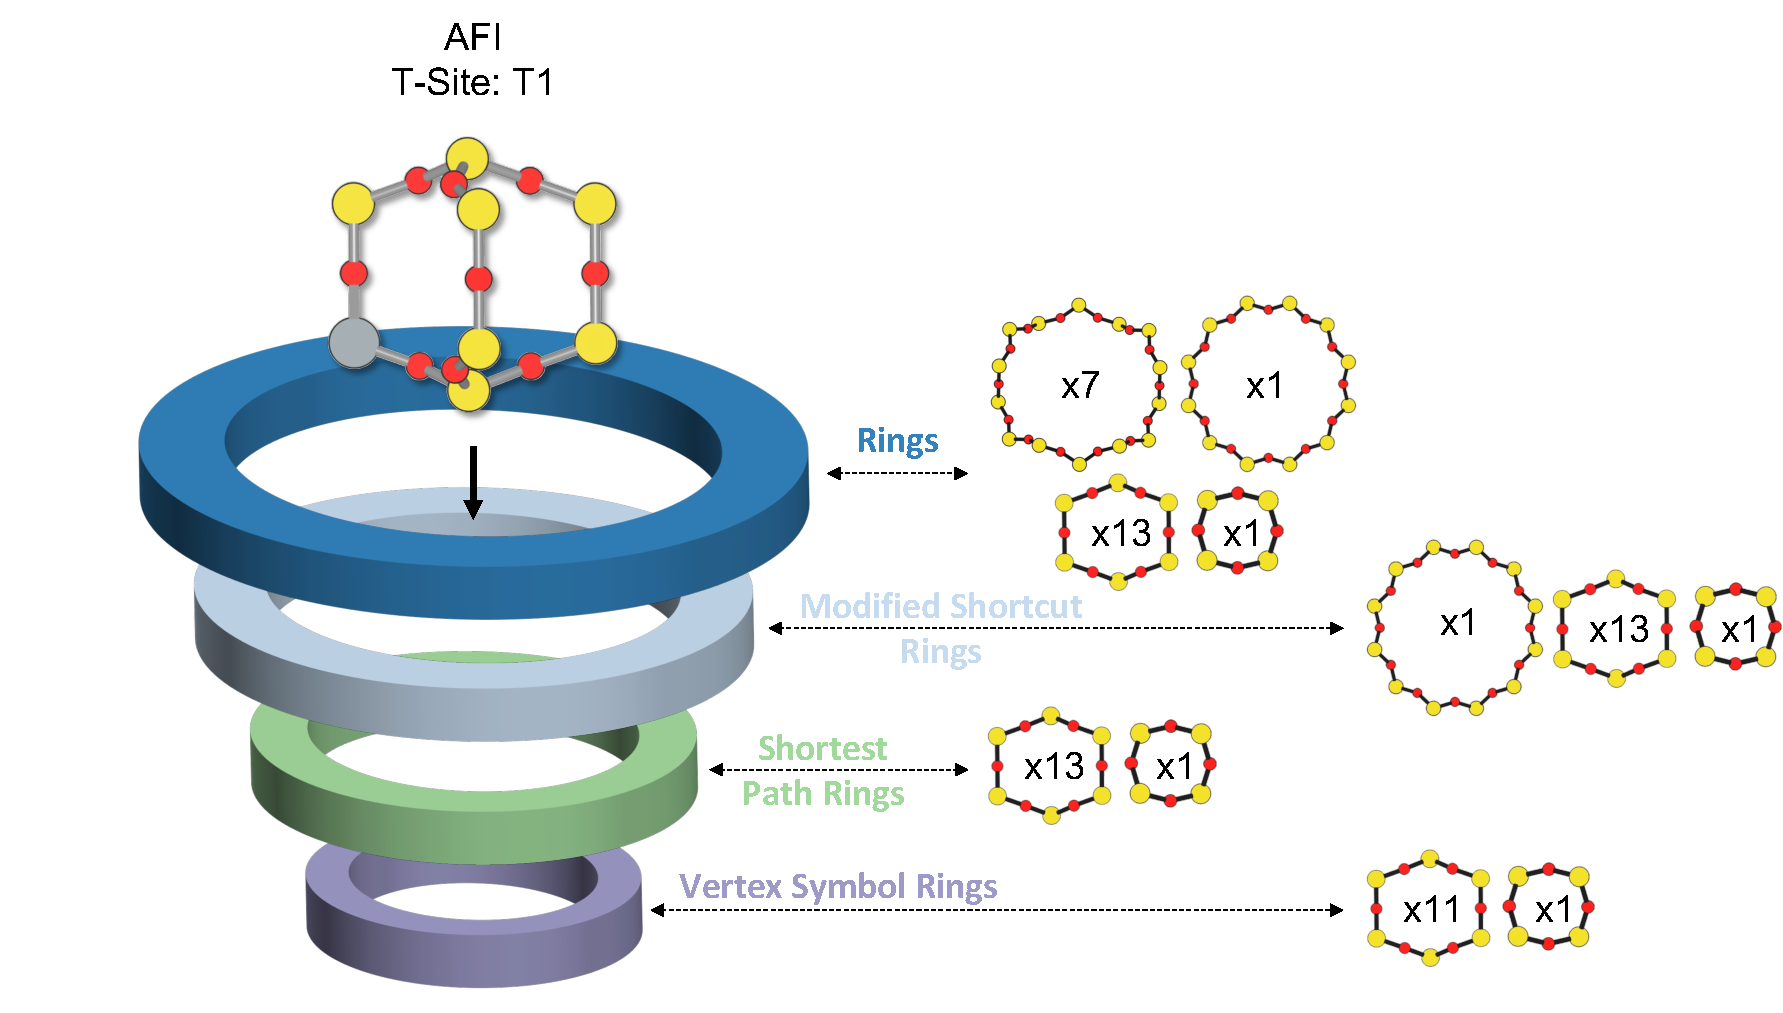
\includegraphics[width=\textwidth]{figures/chapter-3/afi-funnel.pdf}
\caption{Diagram shwoing the ring counts of each size ring that pass through the single symmetry distinct T-site in AFI for each of the various ring finding conventions. \label{fig:afi-funnel}}
\end{figure}
\end{figure}

With an understanding of how we characterize T-sites by counting the rings that pass through them, \cref{tab:uninodal} shows the ring index for a selection of T-sites from uninodal (containing only one symmetry distinct T-site) frameworks. This table highlights the differences in ring counts found with each convention, and shows that in general as you move from left to right across the table the largest ring size found decreases. The results in the shortest path column were found using ZSE, but agree directly with the results shown by Sastre and Corma \cite{sastre-topological-2009}. The results in the vertex symbol rings column were also found with ZSE, and agree directly with the vertex symbols listed on the IZA Database website \cite{baerlocher-database-nodate}.  

\begin{table}
\centering
\begin{threeparttable}
\caption{Comparison of ring indices for the T-sites in various uninodal zeolite frameworks. \label{tab:uninodal}}
{\scriptsize
\begin{tabular}{lllll}
\hline
Framework & Rings & This Work & Shortest Path Rings \cite{sastre-topological-2009} & Vertex Symbol Rings \cite{baerlocher-database-nodate}\\
\hline
ABW & 4\(_{\text{2}} \cdot\)6\(_{\text{3}} \cdot\)8\(_{\text{4}}\) & 4\(_{\text{2}} \cdot\)6\(_{\text{3}} \cdot\)8\(_{\text{4}}\) & 4\(_{\text{2}} \cdot\)6\(_{\text{3}} \cdot\)8\(_{\text{4}}\) & 4\(_{\text{2}} \cdot\)6\(_{\text{3}} \cdot\)8\(_{\text{2}}\)\\
ACO & 4\(_{\text{3}} \cdot\)6\(_{\text{3}} \cdot\)8\(_{\text{6}} \cdot\)10\(_{\text{15}}\) & 4\(_{\text{3}} \cdot\)8\(_{\text{6}}\) & 4\(_{\text{3}} \cdot\)8\(_{\text{6}}\) & 4\(_{\text{3}} \cdot\)8\(_{\text{6}}\)\\
AFI & 4\(_{\text{1}} \cdot\)\(_{\text{13}} \cdot\)12\(_{\text{1}} \cdot\)14\(_{\text{7}}\) & 4\(_{\text{1}} \cdot\)6\(_{\text{13}} \cdot\)12\(_{\text{1}}\) & 4\(_{\text{1}} \cdot\)6\(_{\text{13}}\) & 4\(_{\text{1}} \cdot\)6\(_{\text{11}}\)\\
ANA & 4\(_{\text{2}} \cdot\)6\(_{\text{2}} \cdot\)8\(_{\text{16}}\) & 4\(_{\text{2}} \cdot\)6\(_{\text{2}} \cdot\)8\(_{\text{16}}\) & 4\(_{\text{2}} \cdot\)6\(_{\text{2}} \cdot\)8\(_{\text{16}}\) & 4\(_{\text{2}} \cdot\)6\(_{\text{2}} \cdot\)8\(_{\text{8}}\)\\
ATO & 4\(_{\text{1}} \cdot\)6\(_{\text{9}} \cdot\)8\(_{\text{8}} \cdot\)12\(_{\text{20}}\) & 4\(_{\text{1}} \cdot\)6\(_{\text{9}} \cdot\)12\(_{\text{20}}\) & 4\(_{\text{1}} \cdot\)6\(_{\text{9}}\) & 4\(_{\text{1}} \cdot\)6\(_{\text{9}}\)\\
BCT & 4\(_{\text{1}} \cdot\)6\(_{\text{6}} \cdot\)8\(_{\text{20}}\) & 4\(_{\text{1}} \cdot\)6\(_{\text{6}} \cdot\)8\(_{\text{12}}\) & 4\(_{\text{1}} \cdot\)6\(_{\text{6}}\) & 4\(_{\text{1}} \cdot\)6\(_{\text{6}}\)\\
CHA & 4\(_{\text{3}} \cdot\)6\(_{\text{1}} \cdot\)8\(_{\text{6}} \cdot\)12\(_{\text{1}}\) & 4\(_{\text{3}} \cdot\)6\(_{\text{1}} \cdot\)8\(_{\text{2}} \cdot\)12\(_{\text{1}}\) & 4\(_{\text{3}} \cdot\)6\(_{\text{1}} \cdot\)8\(_{\text{2}}\) & 4\(_{\text{3}} \cdot\)6\(_{\text{1}} \cdot\)8\(_{\text{2}}\)\\
DFT & 4\(_{\text{2}} \cdot\)6\(_{\text{6}} \cdot\)8\(_{\text{10}} \cdot\)10\(_{\text{10}}\) & 4\(_{\text{2}} \cdot\)6\(_{\text{6}} \cdot\)8\(_{\text{10}}\) & 4\(_{\text{2}} \cdot\)6\(_{\text{6}} \cdot\)8\(_{\text{10}}\) & 4\(_{\text{2}} \cdot\)6\(_{\text{4}} \cdot\)8\(_{\text{6}}\)\\
GIS & 4\(_{\text{3}} \cdot\)8\(_{\text{4}}\) & 4\(_{\text{3}} \cdot\)8\(_{\text{4}}\) & 4\(_{\text{3}} \cdot\)8\(_{\text{4}}\) & 4\(_{\text{3}} \cdot\)8\(_{\text{4}}\)\\
GME & 4\(_{\text{3}} \cdot\)6\(_{\text{1}} \cdot\)8\(_{\text{6}} \cdot\)12\(_{\text{7}}\) & 4\(_{\text{3}} \cdot\)6\(_{\text{1}} \cdot\)8\(_{\text{2}} \cdot\)12\(_{\text{1}}\) & 4\(_{\text{3}} \cdot\)6\(_{\text{1}} \cdot\)8\(_{\text{2}}\) & 4\(_{\text{3}} \cdot\)6\(_{\text{1}} \cdot\)8\(_{\text{2}}\)\\
MER & 4\(_{\text{3}} \cdot\)8\(_{\text{4}} \cdot\)10\(_{\text{10}} \cdot\)14\(_{\text{14}}\) & 4\(_{\text{3}} \cdot\)8\(_{\text{4}}\) & 4\(_{\text{3}} \cdot\)8\(_{\text{4}}\) & 4\(_{\text{3}} \cdot\)8\(_{\text{4}}\)\\
MON & 4\(_{\text{1}} \cdot\)5\(_{\text{5}} \cdot\)8\(_{\text{6}}\) & 4\(_{\text{1}} \cdot\)5\(_{\text{5}} \cdot\)8\(_{\text{6}}\) & 4\(_{\text{1}} \cdot\)5\(_{\text{5}} \cdot\)8\(_{\text{6}}\) & 4\(_{\text{1}} \cdot\)5\(_{\text{4}} \cdot\)8\(_{\text{4}}\)\\
NPO & 3\(_{\text{1}} \cdot\)6\(_{\text{6}} \cdot\)12\(_{\text{40}}\) & 3\(_{\text{1}} \cdot\)6\(_{\text{6}} \cdot\)12\(_{\text{40}}\) & 3\(_{\text{1}} \cdot\)6\(_{\text{6}}\) & 3\(_{\text{1}} \cdot\)6\(_{\text{6}}\)\\
\hline
\end{tabular}
\begin{tablenotes}
Vertex symbols have been represented in ring index format for ease of comparison.
}
\end{tablenotes}
\end{threeparttable}
\end{table}

Next, we take an in-depth look at the ring counts for a framework with multiple symmetry distinct T-sites, to show how a ring index can provide information about the local environment around a T-site, and help differentiate them. MOZ is a zeolite framework containing 4-, 6-, 8-, 10-, 12-, 14-, and 18-MRs, 6 symmetry distinct T-sites, and two distinct 12-MR channels. \cref{tab:moz} shows the ring index for each T-site using each ring finding method.

\begin{table}
\centering
\begin{threeparttable}
\caption{Ring indices for each distinct T-site in the MOZ framework using each ring counting convention. \label{tab:moz}}
{\scriptsize
\begin{tabular}{lllll}
\hline
T-Site & Rings & This Work & Shortest Path Rings & Vertex Symbol Rings\\
\hline
T1 & 4\(_{\text{3}} \cdot\)6\(_{\text{2}} \cdot\)8\(_{\text{7}} \cdot\)10\(_{\text{7}} \cdot\)18\(_{\text{5}}\) & 4\(_{\text{3}} \cdot\)6\(_{\text{2}} \cdot\)8\(_{\text{3}}\) & 4\(_{\text{3}} \cdot\)6\(_{\text{2}} \cdot\)8\(_{\text{3}}\) & 4\(_{\text{3}} \cdot\)6\(_{\text{2}} \cdot\)8\\
T2 & 4\(_{\text{3}} \cdot\)6\(_{\text{2}} \cdot\)8\(_{\text{7}} \cdot\)10\(_{\text{7}} \cdot\)14\(_{\text{5}}\) & 4\(_{\text{3}} \cdot\)6\(_{\text{2}} \cdot\)8\(_{\text{3}}\) & 4\(_{\text{3}} \cdot\)6\(_{\text{2}} \cdot\)8\(_{\text{3}}\) & 4\(_{\text{3}} \cdot\)6\(_{\text{2}} \cdot\)8\\
T3 & 4\(_{\text{3}} \cdot\)6\(_{\text{2}} \cdot\)8\(_{\text{5}} \cdot\)10\(_{\text{4}} \cdot\)12\(_{\text{4}} \cdot\)14\(_{\text{5}}\) & 4\(_{\text{3}} \cdot\)6\(_{\text{2}} \cdot\)8\(\cdot\)12\(_{\text{4}}\) & 4\(_{\text{3}} \cdot\)6\(_{\text{2}} \cdot\)8 & 4\(_{\text{3}} \cdot\)6\(_{\text{2}} \cdot\)8\\
T4 & 4\(_{\text{2}} \cdot\)6\(\cdot\)8\(_{\text{6}} \cdot\)10\(_{\text{6}} \cdot\)12\(\cdot\)18\(_{\text{26}}\) & 4\(_{\text{2}} \cdot\)6\(\cdot\)8\(_{\text{6}} \cdot\)12 & 4\(_{\text{2}} \cdot\)6\(\cdot\)8\(_{\text{6}} \cdot\)12 & 4\(_{\text{2}} \cdot\)6\(\cdot\)8\(_{\text{6}} \cdot\)12\\
T5 & 4\(_{\text{2}} \cdot\)6\(\cdot\)8\(_{\text{7}} \cdot\)10\(_{\text{6}} \cdot\)14\(_{\text{18}}\) & 4\(_{\text{2}} \cdot\)6\(\cdot\)8\(_{\text{7}}\) & 4\(_{\text{2}} \cdot\)6\(\cdot\)8\(_{\text{7}}\) & 4\(_{\text{2}} \cdot\)6\(\cdot\)8\(_{\text{7}}\)\\
T6 & 4\(_{\text{2}} \cdot\)6\(\cdot\)8\(_{\text{3}} \cdot\)10\(_{\text{2}} \cdot\)12\(_{\text{8}} \cdot\)14\(_{\text{18}}\) & 4\(_{\text{2}} \cdot\)6\(\cdot\)8\(_{\text{3}} \cdot\)12\(_{\text{8}}\) & 4\(_{\text{2}} \cdot\)6\(\cdot\)8\(_{\text{3}}\) & 4\(_{\text{2}} \cdot\)6\(\cdot\)8\(_{\text{3}}\)\\
\hline
\end{tabular}
\begin{tablenotes}
Vertex symbols have been represented in ring index format for ease of comparison.
}
\end{tablenotes}
\end{threeparttable}
\end{table}

\cref{fig:moz} shows the T-site locations inside a 2-dimensional view of the framework. If you were interested in which T-sites have access to the 12-MR channels, the shortest path rings and vertex symbol rings would only suggest T3 participates in the 12-MR rings. However, the all rings convention and the modified shortcut convention both identify T4 and T6 as participating in the 12-MR channels as highlighted in \cref{fig:moz}. 

\begin{figure}
\begin{figure}[H]
\centering
\includegraphics[width=\textwidth]{figures/chapter-3/moz.pdf}
\caption{Cutout of the MOZ framework showing two 12-MR channels, with an example of each distinct T-site highlighted. T1: navy, T2: green, T3: orange, T4: purple, T5: blue, and T6: red. As shown, T3, T4, and T6 are all associated with the 12-MR channels, while T1, T2, and T5 are not connected to the 12-MR channels. \label{fig:moz}}
\end{figure}
\end{figure}

We next used ZSE to find the rings associated with every symmetry distinct T-site in every framework across the IZA Database using each of the four ring counting conventions. For each T-site we used the rings to generate a ring index, and \cref{fig:unique-ts} shows how many unique ring indices are present when using each of the ring counting conventions. The plot follows intuition with the number of unique ring indices decreasing as we use more restrictive ring counting conventions, because fewer rings are found providing less room for differentiation. This raises the question, if you want to ascertain chemical or physical properties about a T-site based on its ring count, and differentiate these T-sites from other similar but distinct T-sites, which ring counting convention will suffice? The answer will depend on what level of detail is desired. Larger rings can be found with the standard shortcut definition, while rings traversing other stacked rings will be excluded with our modified shortcut definition. The shortest path definition and vertex symbol rings will provide the most localized information about a T-site. 

\begin{figure}
\begin{figure}[H]
\centering
\includegraphics[width=\textwidth]{figures/chapter-3/unique-ts.pdf}
\caption{Number of unique T-site ring indices when classified by the rings passing through them using the various ring counting conventions. There are 1460 T-sites across all the frameworks in the IZA Database. As we move from less restrictive to more restrictive (left to right) ring counting conventions, the number of unique ring indices decreases. \label{fig:unique-ts}}
\end{figure}
\end{figure}

To further compare the ring counting conventions, we show a distribution of the number of T-sites containing each size ring between 3- and 18-MR in \cref{fig:tsite-frequency} (right). This plot highlights that more T-sites contain larger sized rings when using the basic definition of a shortcut, and at smaller rings sizes (\textless6-MR) all the ring counting conventions return the same results.  To further emphasize these results, we have provided a cumulative distribution of the same data normalized to the maximum 'rings' value in \cref{fig:tsite-frequency}. At 6-MRs is where we see the cumulative distribution functions deviate from each other. The largest deviation takes place at 12-MRs, and the cumulative distributions start to level out at larger ring sizes. 

\begin{figure}
\begin{figure}[H]
\centering
\includegraphics[width=\textwidth]{figures/chapter-3/dist-cumudist.pdf}
\caption{Frequency of T-sites accross all IZA frameworks containing ring sizes between 3- and 18-MR (left), and cumulative distribution of T-sites containing each ring size normalized to the final 'rings' value (right). \label{fig:tsite-frequency}}
\end{figure}
\end{figure}

To complete the comparison of ring counting conventions, we have developed a method to determine their similarity. We do this by comparing the ring index for a T-site using each convention, where the similarity of the ring indices is scored with \cref{eq:similarity}. In this equation, sr is the number of similar rings that are found in both counting conventions, and mr is the maximum number of rings found by either convention. For example: the ring index of AFI using the classic shortcut definition and the shortest path definition are 4\(\cdot\)6\(_{\text{13}} \cdot\)12\(\cdot\)14\(_{\text{7}}\) and 4\(\cdot\)6\(_{\text{13}} \cdot\). The number of similar rings found by both conventions is 14, and the maximum number of rings found by either convention is 22. This would lead to a similarity score of 0.636. We do this for every T-site between two conventions and average the similarity score to get the results in \cref{fig:similarity}. Down the diagonal each method is compared to itself and clearly has a similarity of 1. The remainder of the table follows intuition, in that the  most restrictive ring counting convention (vertex symbol rings) compared to the least restrictive convention (rings) has the lowest similarity score. The two most similar ring counting methods are our modified shortcut definition and the shortest path rings. 

\begin{equation}\label{eq:similarity}
s = \mathrm{ \frac{sr}{mr} }
\end{equation}

\begin{figure}
\begin{figure}[H]
\centering
\includegraphics[width=\textwidth]{figures/chapter-3/similarity-heat-map.pdf}
\caption{Heat map showing the similarity score for four ring counting methods. Similarity score of 1 means identical set of rings returned, while a similarity of 0 would mean no matching rings are returned. \label{fig:similarity}}
\end{figure}
\end{figure}

The conventional definition of a vertex symbol, which lists pairs of rings along opposite edges of the tetrahedron from smallest to largest, only partially captures  the stereochemistry around a T-site. As an example, \cref{fig:stereo} illustrates the rings associated  with T3, T9, and T1 or MOR, MON, and EON, respectively, all of which share the same 4\(\cdot\)5\(_{\text{2}} \cdot\)5\(\cdot\)8\(_{\text{2}} \cdot\)5\(\cdot\)8\(_{\text{2}}\) vertex symbol. While MOR T3 and EON T9 are similar, MON T1 differs in the location of the 5\(_{\text{2}}\)- and 4-MR edges, as highlighted in the lower panel of \cref{fig:stereo}. To remove this ambiguity, an alternative approach is to list the rings of the vertex symbol by starting with the largest one and systematically adding the remaining rings following the edges of the tetrahedron such that each ring listed is connected to one of the oxygen atoms of the next ring listed. This provides a physical meaning to the order of the vertex symbol rings which accounts for differences in the connectivity of those rings around the T-site. Within this algorithm MOR T3 and EON T9 would be labeled as: 8\(_{\text{2}} \cdot\)8\(_{\text{2}} \cdot\)5\(_{\text{2}} \cdot\)5\(\cdot\)4\(\cdot\)5, and MON T1 as: 8\(_{\text{2}} \cdot\)8\(_{\text{2}} \cdot\)4\(\cdot\)5\(\cdot\)5\(_{\text{2}} \cdot\)5. The difference is subtle but highlights the distinct structural difference between the two types of T-sites that is not otherwise captured by a vertex symbol.  We computed the ordered vertex symbols for  all 1460 T-sites in the IZA Database.  The 649 unique vertex symbols in the database increase to 666 unique ordered vertex symbols. Thus, the consideration of stereochemistry only modestly increases the space of unique  tetrahedral sites.  \cref{tab:ov}  lists some common T-site vertex symbols and associated ordered vertex symbols. Complete results are presented in the Supplementary Information.

\begin{figure}
\begin{figure}[H]
\centering
\includegraphics[width=\textwidth]{figures/chapter-3/stereo.pdf}
\caption{Cutout of the MOR, EON, and MON frameworks that only shows the rings associated with the vertex symbol of T3, T9, and T1 respectively. The 4-MR (green) and 2\texttimes{} 5-MR (teal) that are in swapped positions are highlighted for emphasis. The 4-MR for MON, and the 2\timex 5-MRs for MOR and EON are into the plane, and not easily shown. \label{fig:stereo}}
\end{figure}
\end{figure}

% The structural differences shown in \cref{fig:stereo} that are not able to be captured by the vertex symbol leads us to believe that the vertex symbol is not a complete descriptor, and there is room to define a new descriptor that takes into consideration ring orientation. While a vertex symbol includes the shortest rings connecting the four oxygen atoms adjacent to a T-site, and listing them by size and opposite edges, there is still ambiguity in the exact connectivity of those rings. This has led us to create a new method for listing the rings in the vertex symbol that considers the structural connection of the rings described in \cref{section:ov}. 


\begin{table}
\centering
\begin{threeparttable}
\caption{List of three vertex symbols, the T-sites associated with them, and the representative ordered vertex symbol for those T-sites. \label{tab:ov}}
{\scriptsize
\begin{tabular}{lll}
\hline
Vertex Symbol & Framework T-site & Ordered Vertex Symbol\\
\hline
5\(\cdot\)5\(\cdot\)5\(\cdot\)5\(_{\text{2}} \cdot\)5\(\cdot\)10 & EWS T3 & 10\(\cdot\)5\(_{\text{2}} \cdot\)5\(\cdot\)5\(\cdot\)5\(\cdot\)5\\
 & ITN T9 & 10\(\cdot\)5\(_{\text{2}} \cdot\)5\(\cdot\)5\(\cdot\)5\(\cdot\)5\\
 & ITN T21 & 5\(_{\text{2}} \cdot\)10\(\cdot\)5\(\cdot\)5\(\cdot\)5\(\cdot\)5\\
 & OKO T2 & 10\(\cdot\)5\(_{\text{2}} \cdot\)5\(\cdot\)5\(\cdot\)5\(\cdot\)5\\
 & OKO T5 & 5\(_{\text{2}} \cdot\)10\(\cdot\)5\(\cdot\)5\(\cdot\)5\(\cdot\)5\\
 & PCS T2 & 10\(\cdot\)5\(_{\text{2}} \cdot\)5\(\cdot\)5\(\cdot\)5\(\cdot\)5\\
 & PCS T3 & 5\(_{\text{2}} \cdot\)10\(\cdot\)5\(\cdot\)5\(\cdot\)5\(\cdot\)5\\
 & SFS T10 & 5\(_{\text{2}} \cdot\)10\(\cdot\)5\(\cdot\)5\(\cdot\)5\(\cdot\)5\\
 & SFV T3 & 5\(_{\text{2}} \cdot\)10\(\cdot\)5\(\cdot\)5\(\cdot\)5\(\cdot\)5\\
 & SFV T7 & 5\(_{\text{2}} \cdot\)10\(\cdot\)5\(\cdot\)5\(\cdot\)5\(\cdot\)5\\
 & TUN T10 & 10\(\cdot\)5\(_{\text{2}} \cdot\)5\(\cdot\)5\(\cdot\)5\(\cdot\)5\\
\hline
4\(\cdot\)5\(_{\text{2}} \cdot\)5\(\cdot\)8\(\cdot\)5\(\cdot\)8 & DAC T3 & 5\(_{\text{2}} \cdot\)8\(\cdot\)8\(\cdot\)5\(\cdot\)5\(\cdot\)4\\
 & DAC T4 & 5\(_{\text{2}} \cdot\)8\(\cdot\)8\(\cdot\)5\(\cdot\)5\(\cdot\)4\\
 & EON T10 & 5\(_{\text{2}} \cdot\)8\(\cdot\)8\(\cdot\)5\(\cdot\)5\(\cdot\)4\\
 & EPI T1 & 5\(_{\text{2}} \cdot\)8\(\cdot\)8\(\cdot\)5\(\cdot\)5\(\cdot\)4\\
 & MOR T4 & 5\(_{\text{2}} \cdot\)8\(\cdot\)8\(\cdot\)5\(\cdot\)5\(\cdot\)4\\
 & RSN T4 & 5\(_{\text{2}} \cdot\)8\(\cdot\)5\(\cdot\)5\(\cdot\)8\(\cdot\)4\\
 & VNI T2 & 5\(_{\text{2}} \cdot\)8\(\cdot\)5\(\cdot\)5\(\cdot\)8\(\cdot\)4\\
 & VSV T2 & 5\(_{\text{2}} \cdot\)8\(\cdot\)5\(\cdot\)5\(\cdot\)8\(\cdot\)4\\
 & YFI T9 & 5\(_{\text{2}} \cdot\)8\(\cdot\)8\(\cdot\)5\(\cdot\)5\(\cdot\)4\\
\hline
4\(\cdot\)6\(\cdot\)4\(\cdot\)6\(\cdot\)6\(\cdot\)8 & ATN T1 & 8\(\cdot\)6\(\cdot\)4\(\cdot\)4\(\cdot\)6\(\cdot\)6\\
 & JSN T3 & 8\(\cdot\)6\(\cdot\)6\(\cdot\)4\(\cdot\)4\(\cdot\)6\\
 & PON T1 & 8\(\cdot\)6\(\cdot\)4\(\cdot\)4\(\cdot\)6\(\cdot\)6\\
 & SAS T1 & 8\(\cdot\)6\(\cdot\)4\(\cdot\)4\(\cdot\)6\(\cdot\)6\\
 & ZON T3 & 8\(\cdot\)6\(\cdot\)6\(\cdot\)4\(\cdot\)4\(\cdot\)6\\
\hline
\end{tabular}
\begin{tablenotes}
}
\end{tablenotes}
\end{threeparttable}
\end{table}
\section{Conclusions}
\label{sec:org9840720}
Rings of a graph are well defined; here we identified all rings up to 18-MR in every zeolite framework listed on the IZA Structure Database \cite{baerlocher-database-nodate}. We find that the commonly reported ring sizes in literature and on the IZA website leave out many rings that fit the classical definition of a cycle that do not contain a shortcut. To completely describe the topology of a zeolite these rings are required, however there are often cases where someone might want to consider only a subset of rings of interest. 

We have shown a comparison of three existing conventions used to count rings, and highlighted the differences in rings that are found by each convention. The classic definition of a ring identifies the largest set of ring sizes across all the zeolite frameworks, while the shortest path ring and vertex symbol rings only identify smaller ring sizes. We have provided a modified definition of a shortcut that finds larger rings defining channel openings, but excludes rings that are able to be decomposed into at least one smaller ring. It is important to understand the difference of ring sizes and types found by each convention when discussing the rings of a zeolite framework. A disadvantage to using purely connectivity based definitions of rings is the exclusion of cycles in a framework that behave physicochemically like a ring but contain a shortcut. We have displayed an example case of these geometric rings, and in the future it would be beneficial to develop a computation method of identifying these cycles. 

We describe T-sites in zeolite frameworks by counting all of the rings that pass through the T-site using each of the ring counting conventions described. When using ring finding conventions that find larger rings, we see more diversity in the descriptions of T-sites, which can aid researchers who want to identify similar T-sites across multiple frameworks. We have also shown that the vertex symbol used to describe T-sites leaves out subtle but distinct stereochemical differences in the spatial orientation of the rings around a T-site. To address this shortcoming we have provided a new method for ordering the rings of a vertex symbol that takes into consideration the ring stereochemistry and is able to identify differences in T-sites that have the same vertex symbol. In the future, correlating physicochemical properties of T-sites to the ring descriptors identified with each ring counting convention can help identify sets of frameworks with desired T-site properties. 

\section{Data Statement}
Complete ring finding results are available for download via the Supplementary Information. This folder contains a file for each ring counting convention: all rings, modified shortcut rings, shortest path rings, vertex symbol rings, and ordered vertex symbol rings. These files contain the rings associated with each oxygen atom and T-site in every zeolite framework listed on the IZA Structure Database. 

\section{Acknowledgments}
\label{sec:org5946b2f}

We acknowledge financial support provided by the National Science Foundation under Cooperative Agreement No. EEC-1647722, which is an Engineering Research Center for the Innovative and Strategic Transformation of Alkane Resources. JTC thanks the Arthur J. Schmitt Foundation for financial aid in the form of a PhD fellowship. We thank Dr. Christian Baerlocher for the numerous discussions about the topology of zeolites, and methodologies used by the IZA Structure Database. We thank Dr. German Sastre for providing a copy of zeoTsites to compare results, and for the helpful conversions about use cases and zeolite topology. This research was supported in part by the Notre Dame center for Research Computing through access to high performance computing clusters. 
\backmatter

\bibliographystyle{elsarticle-num}
\bibliography{ref}
\end{document}